% !TeX root = ../thuthesis-example.tex

\chapter{集群故障转移和恢复}

故障转移与恢复是构建高可用性和自动容错能力的核心手段。在上一章中,IoTDB 已经能够全面、精准地诊断出集群的故障,接下来,本章将重点讨论如何有针对性地进行故障恢复和自动转移。

本节描述了在故障检测的基础上,写入请求和查询请求的故障自动转移和恢复能力的设计实现。本节首先描述现有的写入和查询流程,给出容错设计的原则和整体框架,

\section{写入和查询流程概述}

\begin{figure}
  \centering
  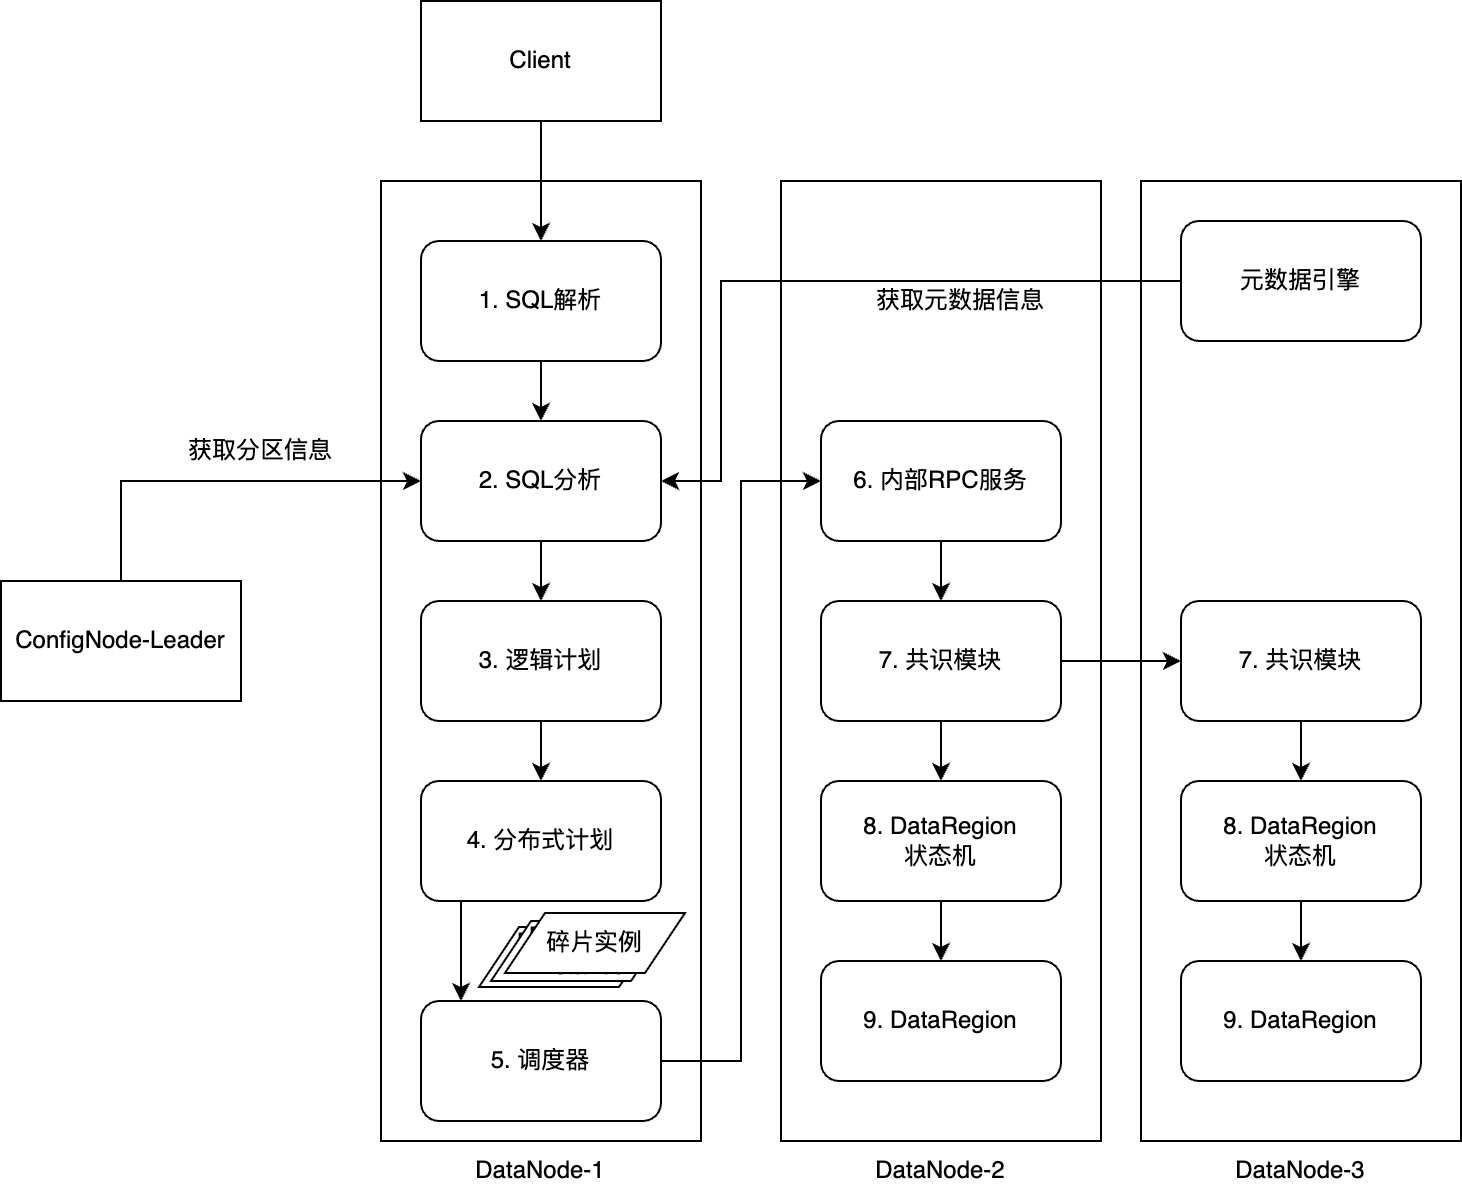
\includegraphics[width=0.99\linewidth]{c04-write-process-redraw.png}
  \caption{IoTDB写入全流程}
  \label{fig:c04-write-process}
\end{figure}

图\ref{fig:c04-write-process}展示了IoTDB现有的写入和查询流程。整个流程涉及三个主要的角色,分别是客户端的会话(Session)、DataNode的协调者(Coordinator)和共识模块的数据副本。Session的主要作用是服务发现、连接状态管理和发送请求,Coordinator负责接受请求并进行处理,共识模块的副本则负责实际数据的写入或者读取。

第一步,客户端可以通过实例化Session对象,和IoTDB服务端的DataNode建立连接,通过SQL等方式发起写入或者查询请求。目前,集群中的所有 DataNode 提供对等的数据写入和查询服务,客户端可以连接至任意 DataNode 发起请求。

第二步,Coordinator会对整个请求进行解析(SQL Parse)。在这个阶段只进行 SQL 语法和格式的校验,确保请求在语法上的正确性。

第三步,Coordinator会进入分析(Analyze)阶段。在本阶段,Coordinator会进行权限校验,确定本次的写入或者查询要访问那些数据,包括识别涉及的时间序列、属性、以及需要查询或写入的数据范围。同时,Coordinator可能需要和ConfigNode 通信,获取最新的集群 Region 分区信息,了解本次访问的数据在哪些 DataNode 上存储。同时,Coordinator也可能需要从其他 DataNode 拉取相关的元数据信息。

第四步,Coordinator根据分析的结果,生成本次请求的逻辑计划,该计划描述了查询或写入操作的逻辑步骤,例如数据的选择、过滤、聚合等,但不涉及具体的物理执行方式。逻辑计划通常以逻辑查询树的形式表示。

第五步,Coordinator在逻辑计划的基础上,考虑到集群中数据的实际分布情况(哪些 Region 存储在哪些 DataNode 上),生成一个分布式执行计划。该计划将逻辑操作分解为可以在不同 DataNode 上并行执行的多个碎片实例 (FragmentInstance)。每个碎片实例负责处理一个特定的数据分区 Region,具备一个ReplicaSet,代表了这个Region的数据副本所在的 所有DataNode。

第六步,Coordinator作为调度器,负责将分布式执行计划中的每个碎片实例调度到相应的 DataNode 上执行。对于某些操作,协调者可能会选择在本地 DataNode 上执行,而对于需要访问其他 DataNode 数据的操作,则会将相应的碎片实例发送到远程 DataNode 执行。如果调度过程中发生错误,协调者可能会尝试重新调度。

第七步,每一个碎片实例最终会被交付给共识层进行执行。共识层会进行相关的读写操作的执行,并且提供数据复制和一致性的保证。以Raft共识协议为例,交给共识层的写入操作会保证被复制给大多数节点执行完成之后才会返回成功写入,交给共识层的读取操作能够保证读到线性一致性的结果。

第八步,共识模块在接收到执行指令后,会调用底层的IoTDB单机存储引擎(采用LSM架构,使用MemTable作为内存结构,使用TsFile\cite{zhao2024apachetsfile}作为持久性外部存储)进行实际的数据写入或读取操作。每个数据副本都由其所在的 DataNode 上的存储引擎进行管理。


\section{写入和查询流程的容错原则和设计}

写入和查询请求的容错原则和设计可以总结为以下几个方面:

1. 利用共识层的多副本能力进行错误转移。当某一个副本失效时,写入和查询请求应当尝试访问其他的健康副本,重试本次的请求直到成功。

2. 利用对副本的知识和集群的已知故障进行最优的执行计划规划和路由规划。如果在规划阶段,已知副本所在的节点出现了进程宕机、服务不可用、网络不可达的情况,那么在计划和规划的阶段就应该避开这些副本,绕开这些故障从而达到最优的执行路由。

3. 一旦发现在规划、执行的阶段中由于故障的原因无法成功完成请求,那么需要尽快通知客户端节点,而不是无用功地在集群内部重试。在通知时需要尽力给出失败的原因和重试的建议,由客户端根据情况决定后续的策略。


\section{协调者规划阶段的容错设计}

规划阶段的容错设计思路是根据集群当前的节点存活情况和副本存活情况,将碎片实例分配到最优的副本上执行。如果找不到任何一个副本来执行这个碎片实例,那么就在规划阶段就报错返回。

\subsection{基于拓扑感知的规划}

IoTDB协调者在进行查询规划和计划生成时,对于根节点碎片实例(Root FragmentInstance)的摆放需要考虑集群的网络拓扑和分区故障。

根节点碎片实例是一种特殊的碎片实例。相较于普通的碎片实例,根节点碎片实例需要负责从其他的分布在不同的存储节点碎片实例中汇聚结果数据,进行最终数据聚合和计算,并将结果发送返回给查询的请求方。由于根节点碎片实例需要和所有的碎片实例进行通信,所以在规划期间,必须保证根节点碎片实例被调度到的节点能够和其他所有碎片实例被调度到的节点的并集联通。


\begin{figure}
  \centering
  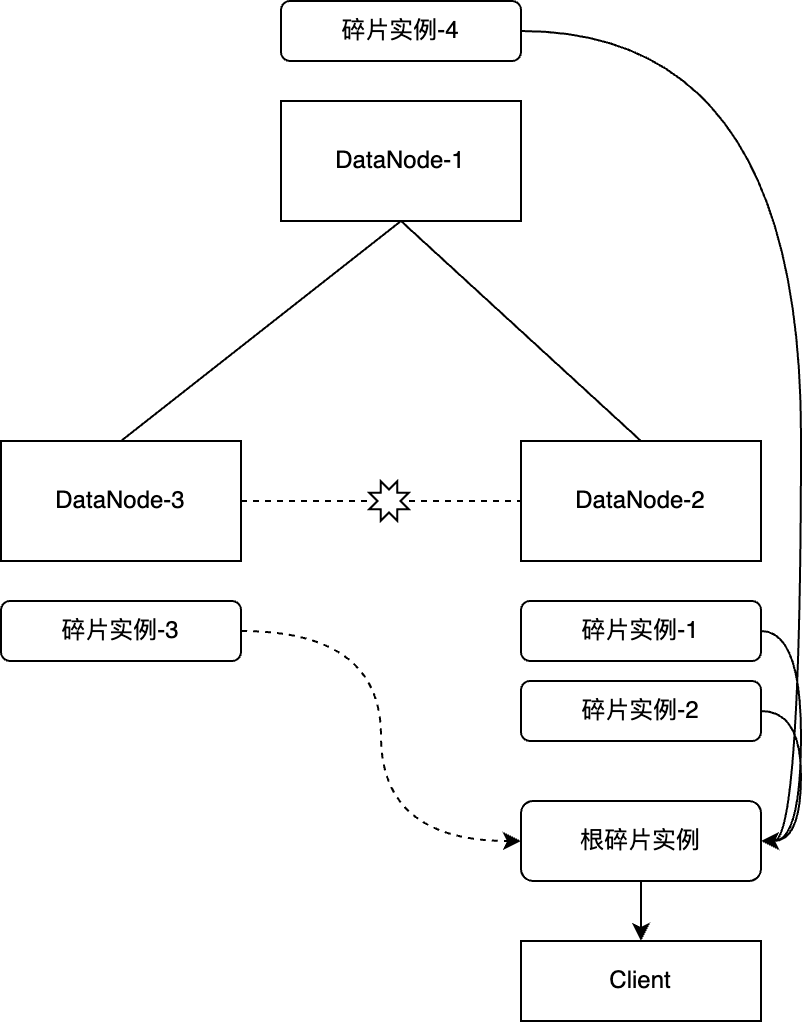
\includegraphics[width=0.7\linewidth]{c04-fi-topology-partition.redraw.png}
  \caption{网络分区下的查询失败情况}
  \label{fig:fi-topology-partition}
\end{figure}

图\ref{fig:fi-topology-partition}展示了非对称网络分区下,根节点的错误放置导致查询失败的一个例子。在这个查询中,一共有四个碎片实例,分别分散在三个DataNode上。其中第一个、第二个碎片实例被调度到了DataNode2上,第三个碎片实例被调度到了DataNode3上,第四个碎片实例被调度到了DataNode1上。

此时,DataNode2和DataNode3之间恰巧出现了非对称网络分区,此时,如果将本次查询的根节点碎片实例调度到DataNode2上,那么这个根节点碎片实例就不能连接上第三个碎片实例,也无法收集这个实例上的数据,最后导致本次查询计划无法执行,最终失败。

因此,在决定查询计划的规划和根节点碎片实例的放置的时候,我们需要考虑节点之间的拓扑结构。根节点的碎片实例放置的DataNode必须具备和所有的碎片实例所在的DataNode都网络可达的性质。算法\ref{alg:find_candidates}给出了根节点碎片实例的放置算法。


再次我们给出基于网络拓扑分区的root fragment instance的算法描述。
\begin{algorithm}
  \caption{查找DataNode和FragmentInstance候选}
  \label{alg:find_candidates}
  \begin{algorithmic}
  \REQUIRE 集群拓扑结构 (连通图), FragmentInstance列表
  \ENSURE DataNode候选列表, FragmentInstance候选列表
  
  \STATE $DataNodeCandidates \leftarrow \emptyset$
  \STATE $FragmentInstanceCandidates \leftarrow \emptyset$
  
  \FOR{每个 DataNode $node$ 在 集群拓扑结构 中}
      \STATE $isCandidate \leftarrow true$
      \FOR{每个 FragmentInstance $instance$ 在 FragmentInstance列表 中}
          \STATE $foundConnection \leftarrow false$
          \FOR{每个 Replica $replica$ 在 $instance.ReplicaSet$ 中}
              \IF{$node$ 和 $replica$ 在 连通图 中连通}
                  \STATE $foundConnection \leftarrow true$
                  \STATE \textbf{break} \COMMENT{找到一个连接即可}
              \ENDIF
          \ENDFOR
          \IF{$foundConnection = false$}
              \STATE $isCandidate \leftarrow false$
              \STATE \textbf{break} \COMMENT{如果和任何ReplicaSet都无法连通,则不是候选}
          \ENDIF
      \ENDFOR
      \IF{$isCandidate = true$}
          \STATE $DataNodeCandidates \leftarrow DataNodeCandidates \cup \{node\}$
      \ENDIF
  \ENDFOR
  
  \FOR{每个 FragmentInstance $instance$ 在 FragmentInstance列表 中}
      \STATE $isCandidate \leftarrow false$
      \FOR{每个 DataNode $candidate$ 在 $DataNodeCandidates$ 中}
          \FOR{每个 Replica $replica$ 在 $instance.ReplicaSet$ 中}
              \IF{$candidate = replica$}
                  \STATE $isCandidate \leftarrow true$
                  \STATE \textbf{break} \COMMENT{找到一个候选DataNode即可}
              \ENDIF
          \ENDFOR
          \IF{$isCandidate = true$}
              \STATE \textbf{break} \COMMENT{找到一个候选DataNode即可}
          \ENDIF
      \ENDFOR
      \IF{$isCandidate = true$}
          \STATE $FragmentInstanceCandidates \leftarrow FragmentInstanceCandidates \cup \{instance\}$
      \ENDIF
  \ENDFOR
  
  \RETURN $DataNodeCandidates$, $FragmentInstanceCandidates$
  \end{algorithmic}
  \end{algorithm}

上述的拓扑感知算法能够使本次的查询成功完成。
此时,根节点碎片实例将会被调度到DataNode1节点上。由于DataNode1分别和DataNode2跟DataNode3之间能够联通,因此即使出现了非对称网络分区的情况下,位于DataNode1上的根节点碎片实例依然能够成功拉取本次查询规划的所有的碎片实例的数据,成功执行本次的查询。


\subsection{基于副本状态的规划}

在协调者进行查询规划时,查询规划器会从ConfigNode Leader这边加载最新的分区信息表,从而保证每一个碎片实例的副本都是最优规划的副本。该步骤包括以下的算法:

1. 规划器会首先选择主副本来执行写入和查询请求。对于RatisConsensus来说,上层应用只能选择主副本来执行写入请求。对于IoTConsensus和IoTConsensusV2来说,虽然每一个副本都能够执行写入请求,但为了避免冲突、提高系统的吞吐,规划器依然会选择ConfigNode Leader指定的主副本来完成数据的写入。

2. 在主副本发生故障时,共识模块和ConfigNode Leader会共同保证主副本的切换。当主副本切换后,规划器就会将后续的查询请求路由到新的主副本上进行执行,从而完成故障转移和容错。在途的写入和查询请求则通过章节\ref{sec:failover-schedule}所描述的调度阶段的容错设计来实现故障的转移和容错。

3. 如果在规划时期,规划器发现某一个Region的所有副本都不可用,那么会直接使这一次查询失败,并返回失败结果给客户端,由客户端对重试的策略作出最终的决策。

在本文的工作之前,规划器并不会使请求立马失败,而是会尝试在每一个副本之间重试,并在每一次重试中间进行一段时间的等待。这种策略常常能够解决副本组暂时性不可用的情况,但是却在网络分区的情况下会进行大量无谓的等待。

\begin{figure}
  \centering
  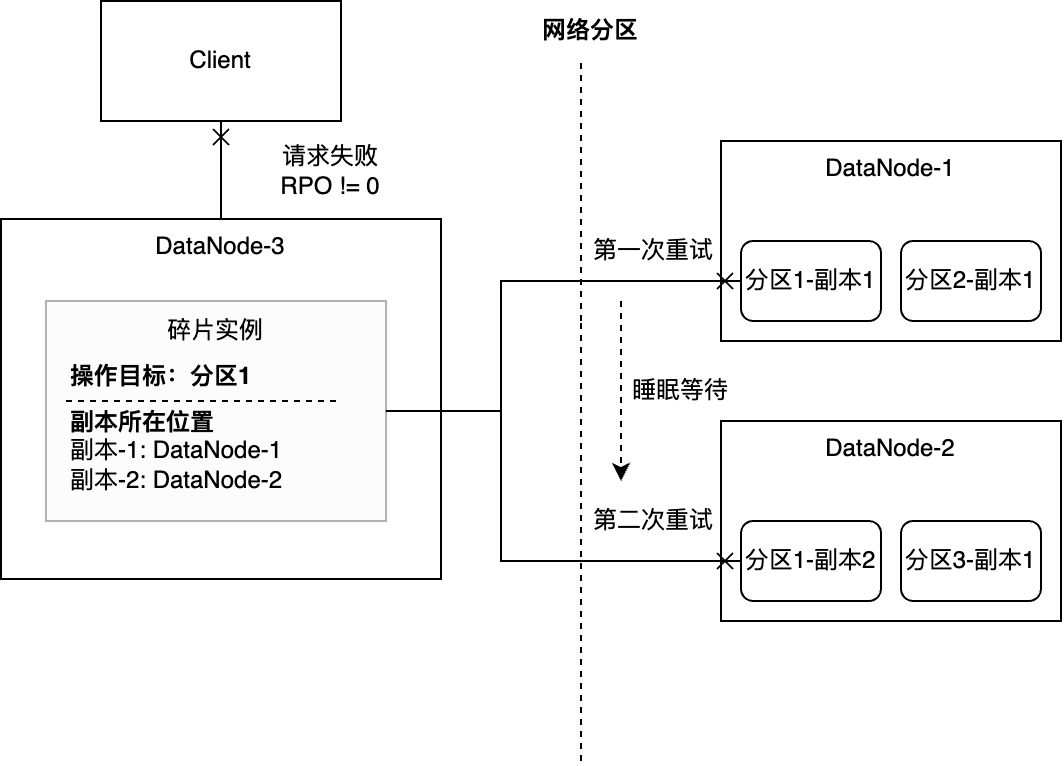
\includegraphics[width=0.9\linewidth]{c04-write-with-topology.redraw.png}
  \caption{网络分区下的写入失败情况}
  \label{fig:c04-write-with-topology}
\end{figure}

图\ref{fig:c04-write-with-topology}中展示了这种大量无谓等待的场景。
在本场景中,DataNode3和DataNode1和DataNode2之间出现了对称网络分区。此时,如果客户端连接上了DataNode3执行写入计划,该计划包含的分区的所有副本都在DataNode1和DataNode2上。
在本文之前,规划器不会立马使这次的写入失败,而是继续交给调度器。调度器会先尝试调度到DataNode1上,但是由于网络分区的问题,本次请求最终会以超时失败。接着,调度器会等待一段时间,接着尝试选择第二个副本执行,再次尝试调度,但本次请求最终依然会因为分区而失败告终。调度器会反复重复上述的重试策略,直到本次的执行超过客户端指定的超时时间,最终返回客户端失败。

这样的规划和调度存在两个问题。在网络分区的情况下,客户端的请求需要经历一个完整的超时重试周期(默认为1分钟)才能被返回,这种无意义的超时和等待会严重影响客户端的吞吐。其次,如果客户端不尝试连接其他的DataNode进行重试,那么本次写入会最终失败,从而导致这部分的数据丢失,影响集群的RPO指标。

因此,本文所提出的容错设计会在发现某一个碎片实例的所有副本位置都不可达的时候直接在规划阶段将这个请求判定为失败,返回客户端该结果,并带上建议的重试节点和方案,由客户端阶段对后续的操作作出决定。


\section{协调者调度阶段的容错设计}\label{sec:failover-schedule}


调度阶段的容错主要面对的故障是在规划阶段未知的故障。对于规划阶段已知的故障,我们可以通过上述章节描述的最优副本选择算法进行规避。但如果一个副本在规划阶段尚且健康存活,但在规划结束开始执行的时候突然出现故障而不可服务请求,那么为了避免本次调度失败而导致请求失败和RPO不为零,我们需要调度阶段的容错能力。

调度阶段的容错的主要方法是对多个副本进行尝试和错误转移。
对于写请求来说,如果写入的目标副本发生了故障,本次写请求可能会出现超时无响应、对应的错误码或者异常抛出,那么此时调度器需要尝试别的副本所在的DataNode进行重试,直到本次请求能够被其他的节点成功写入,或者超过配置的最大写入超时时间而返回。

对于读请求来说,情况则更为复杂,不能在副本级别进行重试,只能在请求级别进行重试。
由于根节点碎片实例需要负责从别的碎片实例中拉取数据,因此根节点在规划阶段就需要了解其他碎片实例的副本所调度的节点。如果某一个碎片实例所调度的副本出现问题,想要转移重试到其他的副本进行调度,那么势必需要通过通知机制让根节点碎片实例了解新的调度情况和副本所在位置。这种通知机制需要极大地修改现有的查询实现和查询结构,因此在实际实现中并不可行。

为此,本文在设计读请求调度阶段的容错能力时,统一在调度错误的时候进行请求级别的重试,即重新规划这个读请求,找到最新的最优副本,然后再进行调度和执行。这种方式通过多次规划和调度的方式,能够发现在第一次规划时期未出现的错误,从而实现容错的目的。

总结来说,调度阶段的容错通过在副本级别重试、在请求级别重试的方法,对集群中那些刚刚产生但尚未被检测的故障进行容错,达到进一步提高可用性的能力。

\section{Session的容错设计}

Session侧的容错设计是IoTDB集群故障转移和恢复能力的最后一块拼图,是IoTDB集群客户端和服务端协同容错的重要组成部分。

Session侧的容错主要目的是实现IoTDB服务的自动发现、自动选择最合适的DataNode完成请求,也是请求的最后兜底方。

Session侧的第一大功能就是服务的自动发现。如前文所述,IoTDB的DataNode在正常情况下都提供了对等的服务,Session可以随机连接到其中的一个DataNode上执行相关的请求和操作。
然而,如果这个被连接的DataNode突发故障,例如进程宕机、因网络分区而导致连接中断、高负载状态下导致资源耗尽而不能很好地提供服务,那么为了保证客户端的请求依然能够被执行、数据能够被写入,Session需要减负检测DataNode故障并且转移到其他健康的DataNode的任务。


在具体实现上,每一个Session启动的时候,都会配置至少一个DataNode节点和ConfigNode的节点。在Session创建之后,会启动一个后台的进程,这个进程会从集群的ConfigNode Leader中定期拉取所有DataNode的列表和其对应的状态。当连接的DataNode发生故障,Session能够通过连接超时、连接通道断开等方式检测出异常的发生,根据列表的顺序不断尝试下一个可用的DataNode,直到能连接到新的DataNode,继续完成请求。


这种切换能力还能实现负载均衡和服务发现。对于高负载的节点,超时会导致Session寻求其他节点的连接,从而在事实上将负载带离这个节点,实现被动负载均衡。同时,如果集群中新增了DataNode,那么后台的拉取线程也能自动发现新的DataNode,无需额外的通知和配置,从而实现服务的自动发现。


Session侧的第二大功能就是自动选择最合适的DataNode完成请求。在集群正常的时期,这一功能将会把客户端的请求引导到最优节点上执行,而在集群故障的时期,这一功能将会把客户端的请求引导到能完成请求的节点上。

在正常时期,Session虽然可以连接任何DataNode完成请求,但是为了减少在集群内部的数据转发,提高集群的整体吞吐和资源利用率,DataNode会在执行完请求之后给出一个重定向的建议。通常,被重定向的节点是Session这些请求所需要写入的Region的主副本所在地。此时,Session通过重定向连接到新的节点上发送请求,就能够直接在新节点上完成数据的写入,避免由其他DataNode节点进行转发。

在故障时期,例如非对称网络分区时期,DataNode的同质性被打破,并非每一个节点的都能同质地接受所有的请求。此时,为了保证集群最大的可用性,将Session的请求尽力的完成,DataNode会在执行请求失败之后给出一个重定向和重试的建议。通常,被重定向的节点拥有更好的网络连通性,能够成功执行所有的碎片实例,从而保障了集群的可用性。

Session侧的最后一大功能就是可用性的最后重试兜底。当请求经过IoTDB服务侧的重试失败返回之后,Session可以进行最后的重试,以期通过这种方式来实现服务的可用。例如,请求的DataNode在发生网络分区之后无法连接其他的节点,则需要发回Session重试,让Session连接其他的节点来完成。再例如,当集群处在变更状态中,ConfigNode对集群副本的状态有滞后,在规划时期出现错误规划,则需要发回Session等待和重试,在下一次重试时期待ConfigNode已经掌握了集群副本的最新状况。



\section{容错的熔断和降级措施}

本章节所依赖的故障转移和恢复大量依赖重试的手段,然而,重试本身可能导致系统的故障更为严重。
当系统故障是由于资源超配而产生时,例如负载过高导致的JVM垃圾回收时间变长、网络已经出现拥塞和超时的等情况下,频繁的重试会进一步加重集群的负担,抢占系统其他请求的存活空间,从而使系统的状态进一步恶化。

我们可以采取对重试进行熔断措施和降级行动来防止恶化。本文所采取的措施如下:

1. 使用指数退避的重试措施。通过在重试之间引入逐渐增加的延迟,默认从100ms开始,每次重试都会翻倍。这种策略能够避免在系统短暂过载的时候引入大量的重试资源。同时,指数退避可以分散重试的时间,避免大量的失败请求因为同一个故障同时重试,导致在服务端形成一个瞬间的请求高峰。如果问题持续存在,逐渐增加的延迟会使得重试的频率降低,减少对已经处于困境的系统的持续冲击。

2. 尽量轮询每一个副本,而不是在一个副本上进行多次重试。如果某个副本本身存在问题(例如,硬件故障、配置错误等),在该副本上进行多次重试很可能仍然会失败,并且会持续消耗该副本的资源,甚至可能导致该副本彻底崩溃。轮询其他副本可以避免将所有压力集中在一个潜在的故障节点上,有助于更均匀地分配集群的负载,避免某些副本压力过大。

3. 设置最大重试次数和最大等待时间,不进行无限期重试,从而确定了一个
当达到最大重试次数后,系统会停止重试,并认为该操作最终失败。这使得系统可以及时地采取其他补救措施,例如返回错误给用户、执行降级逻辑、记录错误日志等,而不是一直停留在重试的状态。


